
\documentclass{report}

\usepackage[utf8]{inputenc}
\usepackage[italian]{babel}
\usepackage{import}
\usepackage{todonotes}
\usepackage{color}
\usepackage{rotating}
\usepackage[hidelinks]{hyperref}
\usepackage{url}
\usepackage{pdfpages}
\usepackage{siunitx}
\usepackage{pdflscape}
\usepackage{subfig}
\usepackage[euler]{textgreek}
\usepackage{mhchem}

\usepackage{multirow}

\usepackage{enumerate} 
\usepackage{amsmath}
\usepackage{amsfonts}

\usepackage[signatures,swapnames,sans]{frontespizio}

\usepackage{geometry}
\geometry{portrait, margin=3cm}
\usepackage{siunitx}
\usepackage{booktabs}

\renewcommand*\figurename{Figura}

\newcommand{\sub}[1]{\textsubscript{#1}}
\newcommand{\super}[1]{\textsuperscript{#1}}
\newcommand{\parallelsum}{\mathbin{\!/\mkern-5mu/\!}}

\newcommand{\Fig}[0]{Fig.}

\usepackage{titlesec}

\titleformat{\chapter}{\normalfont\huge}{}{20pt}{\huge\bfseries}

\linespread{1.3}


%% COMANDI UTILI
%\begin{table}[h]
%	\centering
%	\begin{tabular}{|c|c|c|}
%	\cline{2-3} 
%	\multicolumn{1}{c|}{} & \textbf{Valore nominale} & \textbf{Valore misurato}\\ 
%		%\hline
%		%{} & \textbf{Valore nominale} & \textbf{Valore misurato} \\ 
%		\hline
%		$\mathbf{R_1}$ & \SI{18}{k\ohm} & \SI{17.977}{k\ohm} \\ 
%		\hline
%		$\mathbf{R_2}$& \SI{1.8}{k\ohm} & \SI{1.815}{k\ohm} \\ 
%		\hline
%	\end{tabular}
%\caption{Misure delle resistenze utilizzate per il circuito.}
%\label{table:mis_res}
%\end{table}
%\begin{figure}[h!]
%\centering
%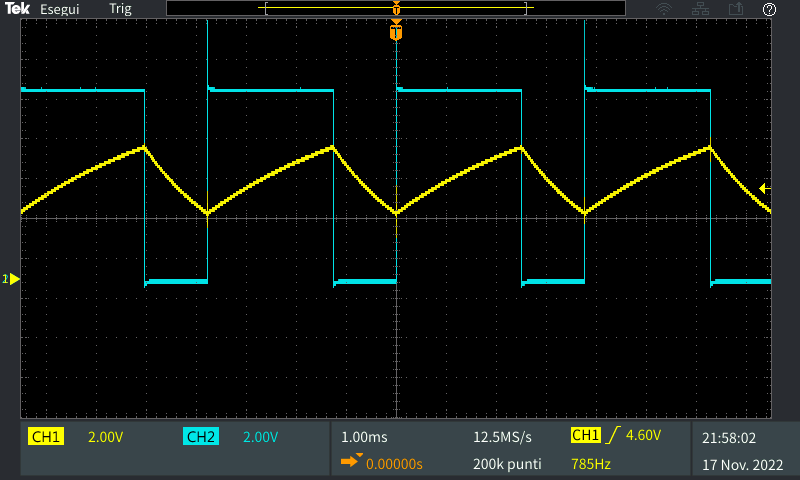
\includegraphics[height=6.5cm]{immagini/TEK00018}\\(a)\\[1ex]
%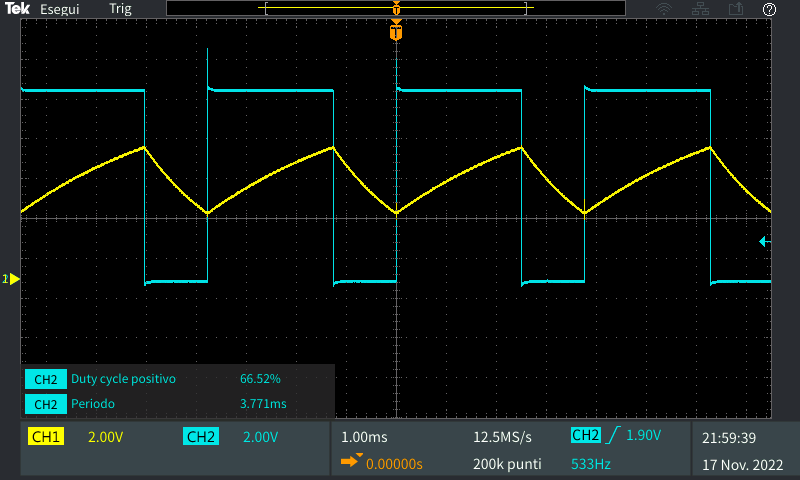
\includegraphics[height=6.5cm]{immagini/TEK00019}\\(b)
%\caption{Risposta del circuito con accoppiamento DC (a) e accoppiamento AC (b).}
%	\label{figura:accopp}
%\end{figure}

\begin{document}
\addtocounter{chapter}{+4}
	\begin{frontespizio}
		\Margini{3cm}{3cm}{3cm}{3cm}
		\Universita{Bergamo}
		\Logo[43.332mm]{unibg-mark}
		\Divisione{Scuola di Ingegneria}
		\Corso[Laurea Magistrale]{Ingegneria Informatica}
		\Titolo{Laboratorio di Elettronica}
		\Sottotitolo{Relazione esperienza di laboratorio 5}
		\Punteggiatura{}
		\NRelatore{Prof.}{Prof.}
		\Relatore{Luigi Gaioni}
		\Candidato[1058231]{Giulia Allievi}
		\Candidato[1059640]{Martina Fanton}
		\Annoaccademico{2022--2023}
		\begin{Preambolo*}
			\usepackage[italian]{babel}
			\usepackage[T1]{fontenc}
			\usepackage[utf8]{inputenc}
			\usepackage{microtype}
			\usepackage{lmodern}
			\graphicspath{{img/}}
			
			\renewcommand{\frontinstitutionfont}{\fontsize{14}{17}\bfseries\scshape}
			\renewcommand{\fronttitlefont}{\fontsize{17}{21}\bfseries\scshape}
			\renewcommand{\frontfootfont}{\fontsize{12}{14}\bfseries\scshape}
		\end{Preambolo*}
	\end{frontespizio}

%----------------------------------------------------------------------------------------
%	PAGINA BIANCA
%----------------------------------------------------------------------------------------
\newpage
\null
\thispagestyle{empty}
\newpage

%----------------------------------------------------------------------------------------
%	INTRO
%----------------------------------------------------------------------------------------
\chapter{Relazione attività di laboratorio 5}
\section*{Introduzione}
In quest'attività di laboratorio abbiamo visto un ultimo circuito monostabile con NE555, successivamente sono state analizzate le altre due configurazioni realizzabili con questo circuito integrato (prima la configurazione bistabile e dopo quella astabile).  \par
La seconda modalità, quella astabile, permette di generare in uscita al pin 3 un'onda quadra le cui caratteristiche dipendono dalla rete collegata all'esterno del circuito integrato. Le connessioni sono illustrate nel datasheet del componente, si riporta di seguito lo schema (figura \ref{figura:datasheet1}).
\begin{figure}[h!]
	\centering
	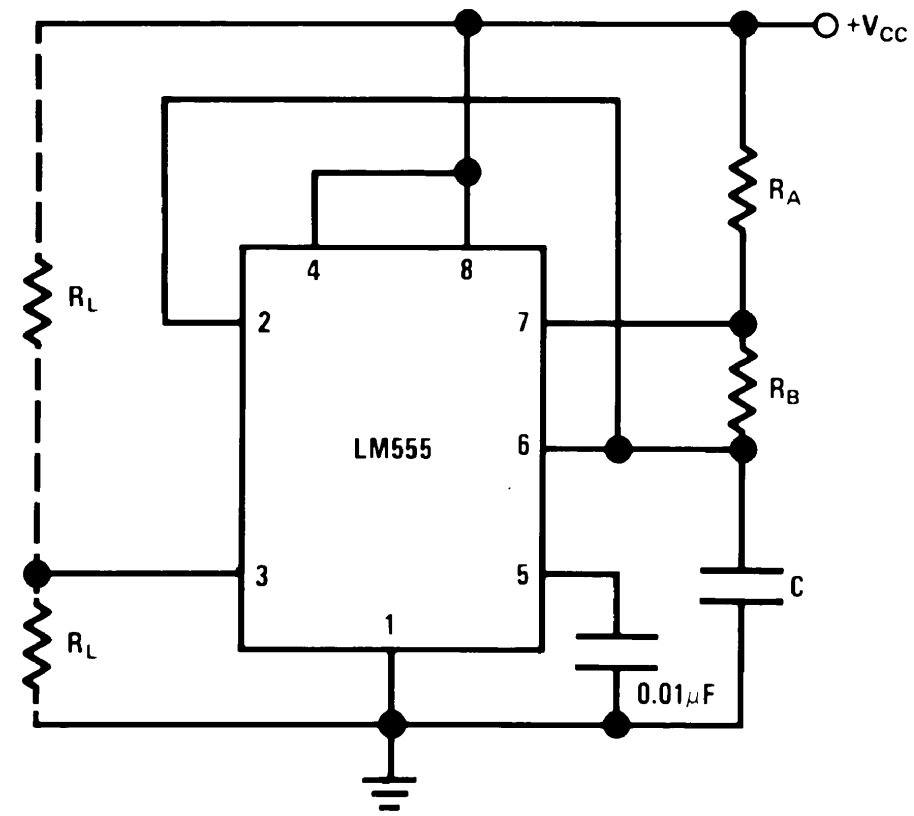
\includegraphics[height=6cm]{immagini/datasheet1}
	\caption{Schema delle connessioni da utilizzare per ottenere un circuito astabile (fonte: \textcolor{blue}{\underline{\href{https://www.ti.com/lit/ds/symlink/lm555.pdf?ts=1667144089940&ref_url=https\%253A\%252F\%252Fwww.ti.com\%252Fproduct\%252FLM555}{datasheet}}}).} % LM o NE ??
	\label{figura:datasheet1}
\end{figure}
\\ La configurazione bistabile invece non è presentata nel datasheet. Questa modalità è utile quando si vuole utilizzare il NE555 come flip-flop set reset. Per ottenerla, è sufficiente utilizzare due resistenze e due pulsanti. Una resistenza è collegata tra i pin 8 e 2, l'altra invece è collegata tra i pin 4 e 8; per quanto riguarda i due pulsanti, uno è collegato tra i pin 2 e 1 e pilota il set, mentre l'altro è connesso ai pin 4 e 1 e comanda il reset. Il pin 8 è collegato all'alimentazione, il pin 1 a massa, il segnale è prelevato al pin 3 e tutti gli altri pin sono lasciati floating. Lo schema si trova nella sezione dedicata all'analisi di questo circuito (sezione \ref{sez2}, figura \ref{figura:schema2}).
\newpage
\section{Circuito 1: NE555 in configurazione monostabile con switch debouncing}
\subsection{Schema del circuito e Funzione di Trasferimento}
Questo circuito è basato principalmente sull'ultimo circuito analizzato nello scorso laboratorio. La differenza più evidente tra i due circuiti è rappresentata dal fatto che questo circuito riceve in ingresso un segnale di trigger generato da un pulsante, mentre il precedente circuito riceveva in ingresso un segnale di trigger fornito da un generatore di forme d'onda. \par
Il circuito in esame, mostrato in figura \ref{figura:schema1}, presenta due resistenze, due capacità e un pulsante. 
\begin{figure}[h!]
	\centering
	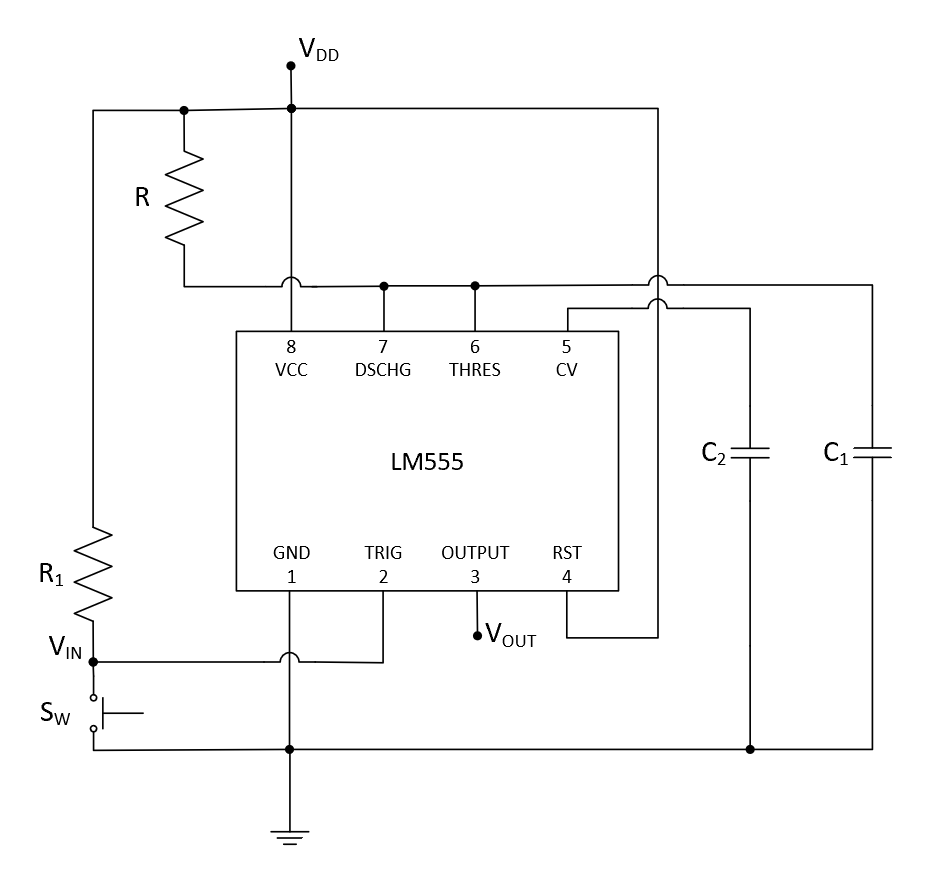
\includegraphics[height=7.5cm]{immagini/schema1}
	\caption{Schema del circuito monostabile con switch debouncing.}
	\label{figura:schema1}
\end{figure}
\\ \noindent La funzione di trasferimento di questo circuito è:
\begin{equation}
	\begin{cases}
		V_{out}= V_{DD}\indent\indent \mathrm{a\;partire\;dalla\;chiusura\;di\;} S_W \mathrm{\;e\;per\;una\;durata\;T\;}\\[5pt]
		V_{out}= 0\indent\indent\indent \mathrm{altrimenti}\\
	\end{cases}
\end{equation}
\subsection{Analisi e dati sperimentali}
Come NE555 è stato scelto un timer della tipologia LM555. Invece per il dimensionamento di questo circuito (in figura \ref{figura:circuito1}) sono state scelte due resistenze da \SI{12}{k\ohm}, la capacità $\mathrm{C_1}$ da \SI{150}{n\farad} e la capacità $\mathrm{C_2}$ da \SI{1}{n\farad}.
\begin{figure}[h!]
	\centering
	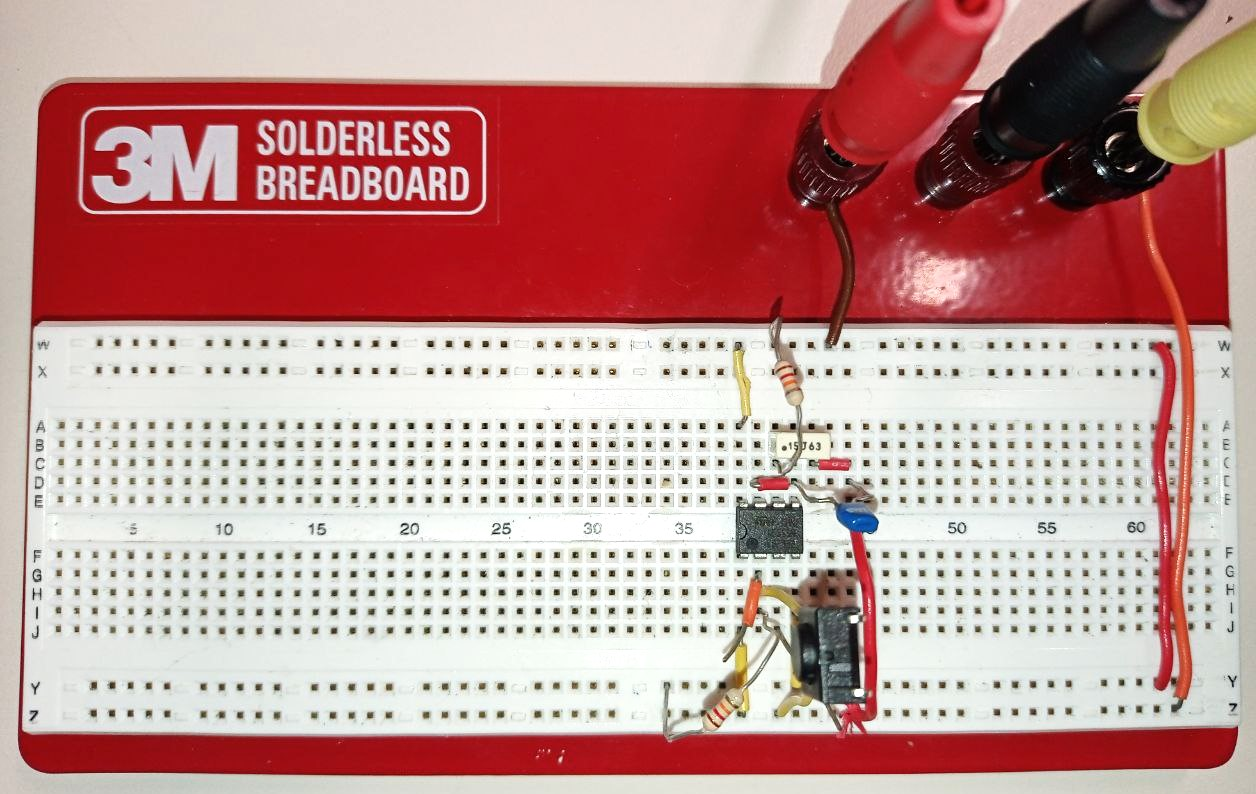
\includegraphics[height=7cm]{immagini/circuito1}
	\caption{Fotografia del circuito monostabile con switch debouncing realizzato in laboratorio.}
	\label{figura:circuito1}
\end{figure}
\newpage
\noindent Nella figura \ref{figura:TEK00016e17} si nota che il segnale in uscita non presenta l'effetto del rimbalzo dell'interruttore e questo è favorito dalla presenza del timer nel circuito.
\begin{figure}[h!]
	\centering
	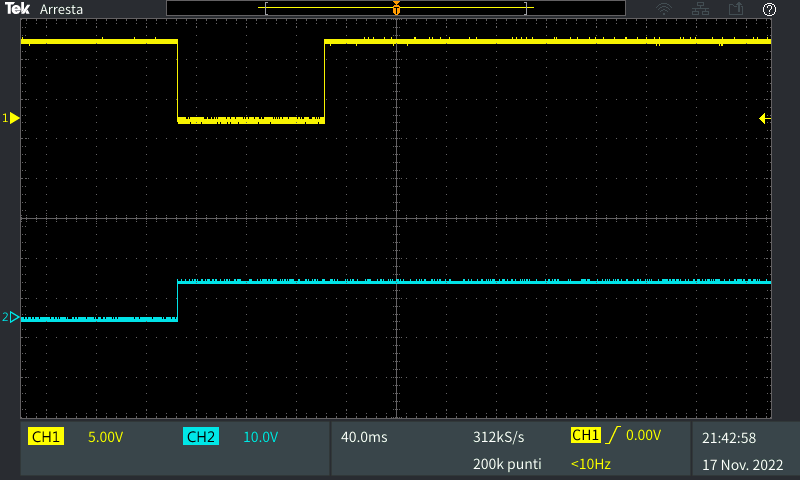
\includegraphics[height=4.6cm]{immagini/TEK00016}
	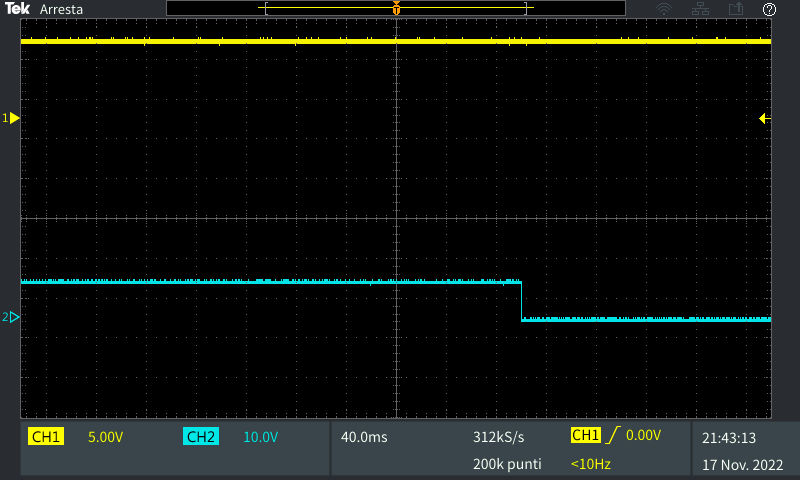
\includegraphics[height=4.6cm]{immagini/TEK00017}
	\caption{Risposta del circuito.}
	\label{figura:TEK00016e17}
\end{figure}
\\Considerando sempre la figura \ref{figura:TEK00016e17}, la durata dell'impulso in ingresso (che, calcolata con l'oscilloscopio, è pari a \SI{120}{m\second}) risulta essere minore della durata dell'impulso in uscita.
\section{Circuito 2: NE555 in configurazione bistabile}\label{sez2}
\subsection{Schema del circuito e Funzione di Trasferimento}
aa
\begin{figure}[h!]
	\centering
	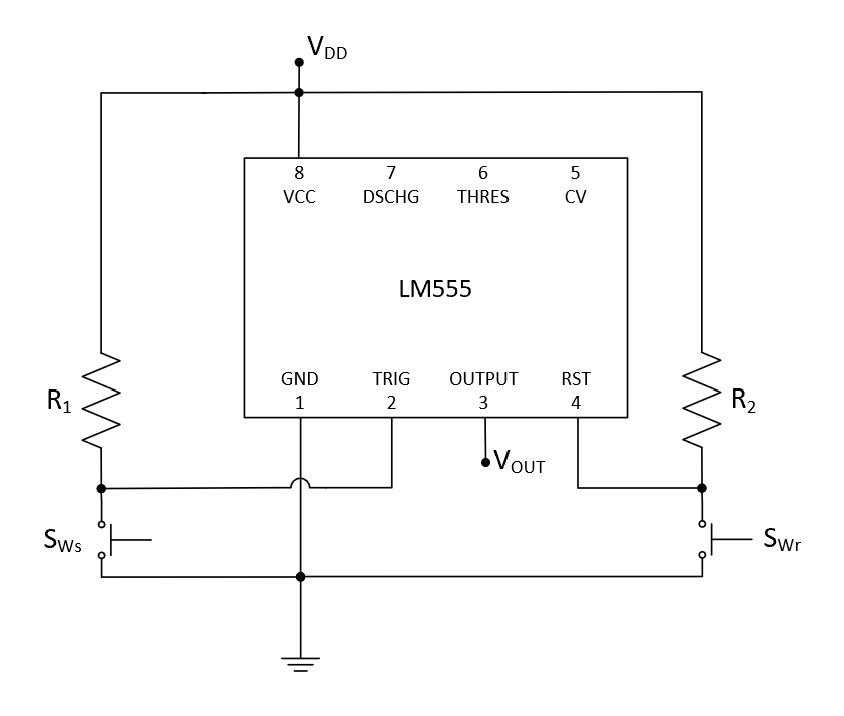
\includegraphics[height=7.5cm]{immagini/schema2}
	\caption{Schema del circuito bistabile.}
	\label{figura:schema2}
\end{figure}
\\ \noindent La funzione di trasferimento di questo circuito è:
\begin{equation}
	\begin{cases}
		V_{out}= V_{DD}\indent\indent \mathrm{a\;partire\;dalla\;pressione\;di\;} S_{Ws} \mathrm{\;fino\;alla\;pressione\;di\;} S_{Wr}\\[5pt]
		V_{out}= 0\indent\indent\indent \mathrm{altrimenti}\\
	\end{cases}
\end{equation}
\subsection{Analisi e dati sperimentali}
\begin{figure}[h!]
	\centering
	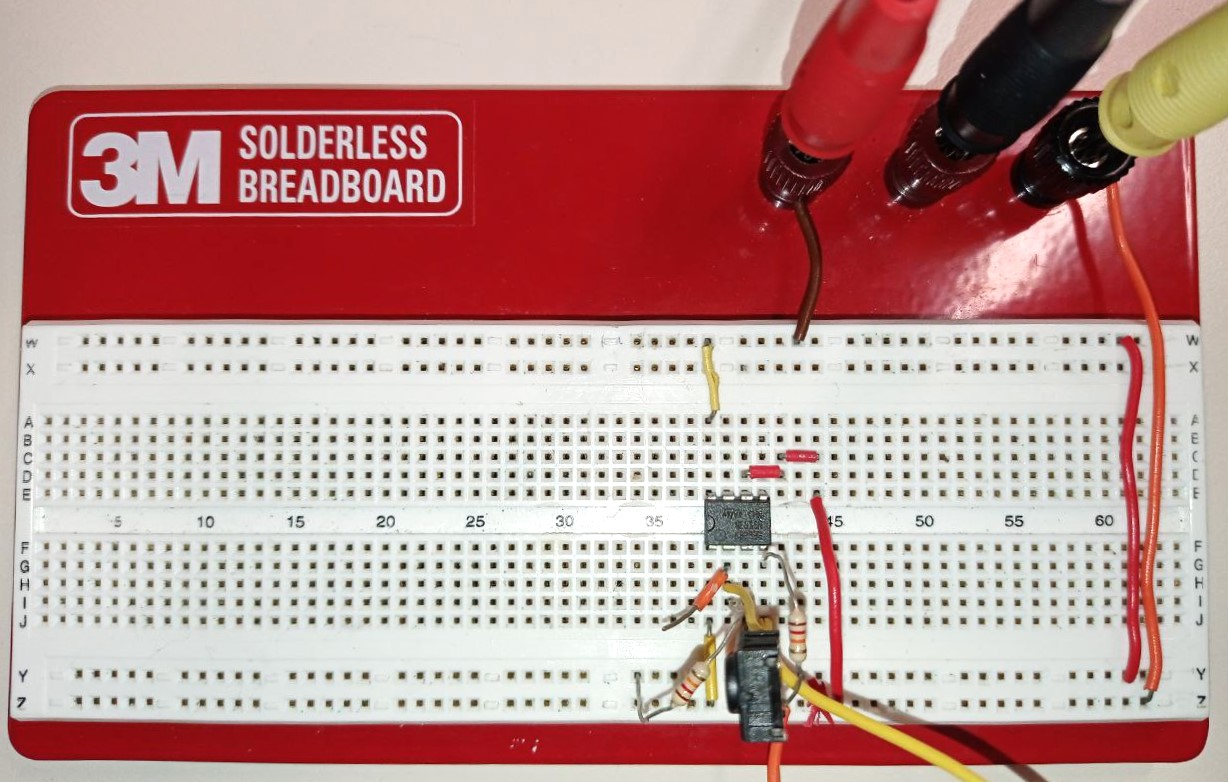
\includegraphics[height=7cm]{immagini/circuito2}
	\caption{Fotografia del circuito bistabile realizzato in laboratorio.}
	\label{figura:circuito2}
\end{figure}
\newpage
\section{Circuito 3: NE555 in configurazione astabile}
\subsection{Schema del circuito e Funzione di Trasferimento}
\begin{figure}[h!]
	\centering
	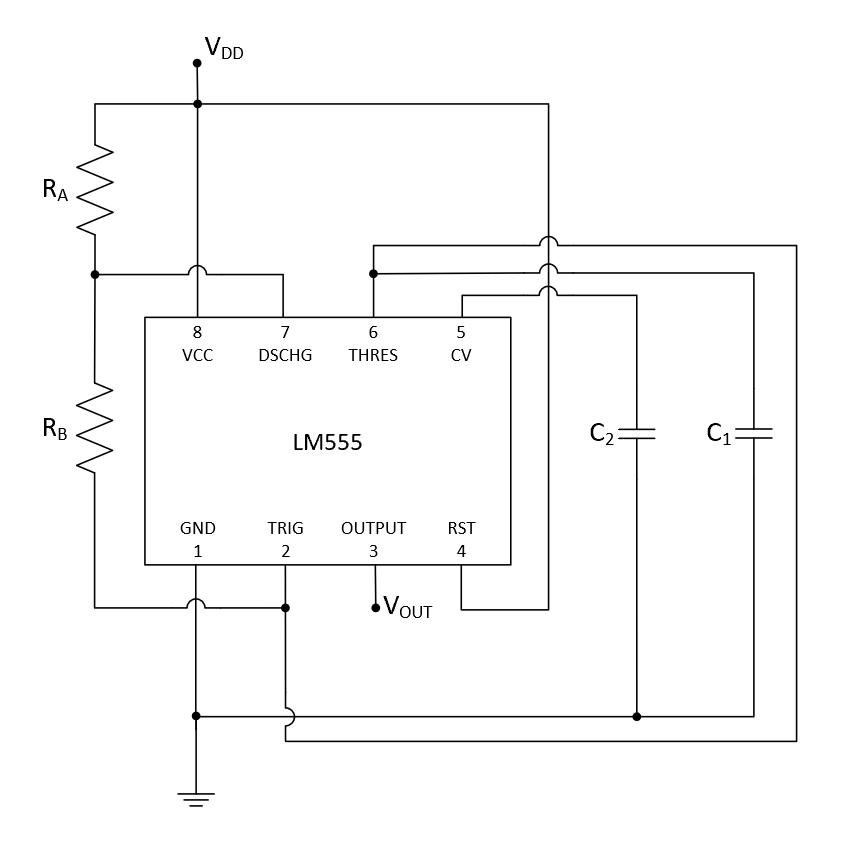
\includegraphics[height=7.5cm]{immagini/schema3}
	\caption{Schema dell'evoluzione del circuito bistabile.}
	\label{figura:schema3}
\end{figure}
\subsection{Analisi e dati sperimentali}
\begin{figure}[h!]
	\centering
	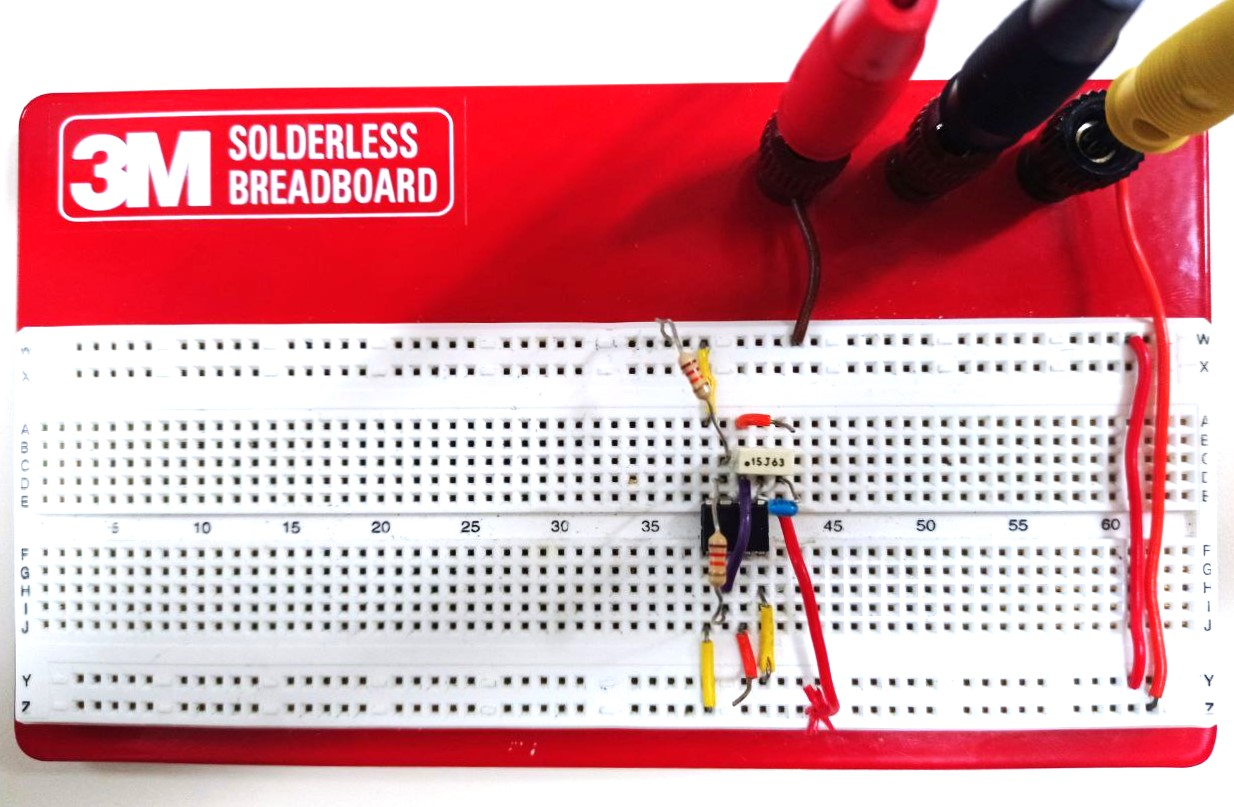
\includegraphics[height=7cm]{immagini/circuito3}
	\caption{Fotografia dell'evoluzione del circuito bistabile realizzata in laboratorio.}
	\label{figura:circuito3}
\end{figure}
\newpage
\section{Circuito 4: Evoluzione del NE555 in configurazione astabile}
\subsection{Schema del circuito e Funzione di Trasferimento}
\begin{figure}[h!]
	\centering
	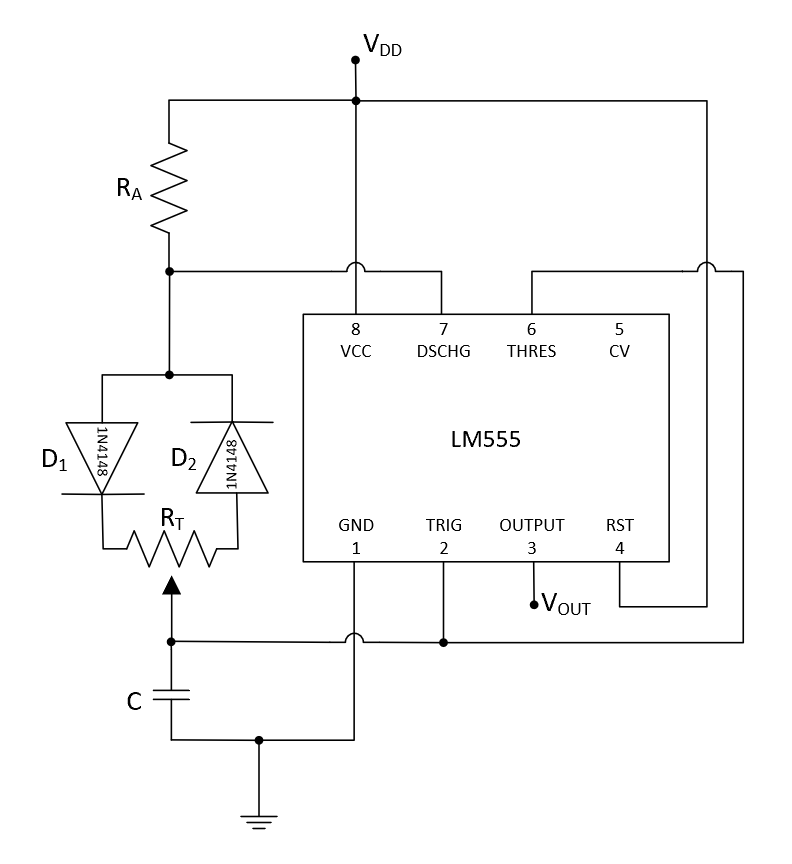
\includegraphics[height=7.5cm]{immagini/schema4}
	\caption{Schema del circuito astabile.}
	\label{figura:schema4}
\end{figure}
\subsection{Analisi e dati sperimentali}
\begin{figure}[h!]
	\centering
	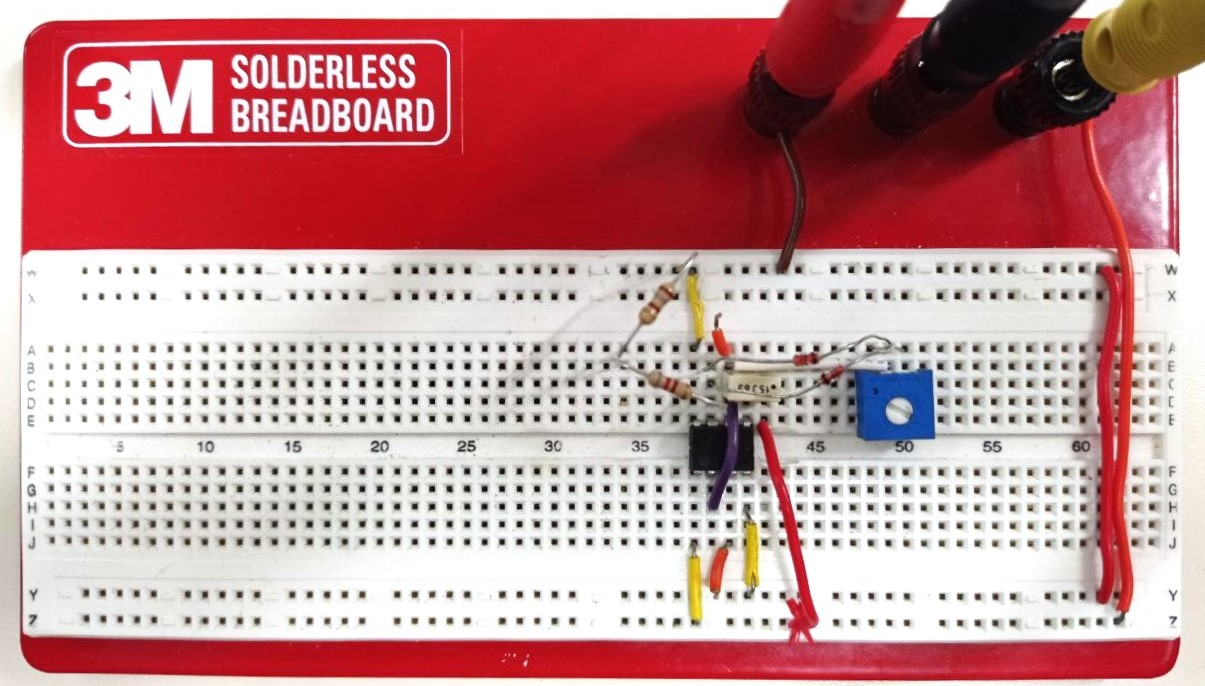
\includegraphics[height=7cm]{immagini/circuito4}
	\caption{Fotografia del circuito astabile realizzato in laboratorio.}
	\label{figura:circuito4}
\end{figure}

%----------------------------------------------------------------------------------------

\end{document}
